\documentclass[11pt,a4paper]{article}

% ---------- Packages ----------
\usepackage[T1]{fontenc}
\usepackage[utf8]{inputenc}
\usepackage{lmodern}
\usepackage[margin=2.5cm]{geometry}
\usepackage{amsmath, amssymb, amsthm}
\usepackage{mathtools}
\usepackage{xcolor}
\usepackage{enumitem}
\usepackage{hyperref}
\hypersetup{colorlinks=true, linkcolor=blue!50!black, urlcolor=blue!50!black, citecolor=blue!50!black}
\usepackage{pgfplots}
\pgfplotsset{compat=1.18}

% ---------- Custom Commands ----------
\newcommand{\E}{\mathbb{E}}
% Indicator macro taking argument: \ind{condition}
\newcommand{\ind}[1]{\mathbf{1}_{\{#1\}}}

% List spacing tweaks
\setlist[enumerate,1]{label=\textbf{\arabic*.}, leftmargin=1.1em}
\setlist[enumerate,2]{label=\alph*), leftmargin=1.5em}

% Optional solution environment
\newif\ifshowsolutions
% Toggle solutions: set to \showsolutionstrue or leave false
\showsolutionstrue % comment this line to hide solutions

\newenvironment{solution}{\par\medskip\noindent\textbf{Solution. }\begingroup}{\endgroup\medskip}

\title{ICE, PDP, ALE}

\date{}

\begin{document}
\maketitle
% \vspace{-1em}\hrulefill\\[0.8em]

\section*{Exercise}
Consider the model
\[
\hat f(x_1,x_2) = 3 \; - 8 x_1 + 16 x_1\, \ind{x_2=\text{``b''}},
\]
with $x_1 \sim \mathrm{Unif}(-1,1)$, $x_2 \in \{\text{``a''},\text{``b''}\}$, and $\Pr(x_2=\text{``b''}) = 0.5$.

\begin{enumerate}
  \item \textbf{ICE curves for $x_1$.}
  \begin{enumerate}
    \item Express the ICE curve for $x_1$ when $x_2=\text{``a''}$ over $t\in[-1,1]$.
    \item Express the ICE curve for $x_1$ when $x_2=\text{``b''}$ over $t\in[-1,1]$.
    \item Determine whether the two ICE curves intersect in $[-1,1]$ and, if so, report the intersection point.
  \end{enumerate}

  \item \textbf{Partial dependence of $x_1$.}
  \begin{enumerate}
    \item Derive the univariate partial dependence function $\mathrm{PD}_{x_1}(t)=\E_{X_2}[\hat f(t,X_2)]$.
    \item In a single sketch, overlay the two ICE curves from item 1 with $\mathrm{PD}_{x_1}(t)$ for $t\in[-1,1]$.
    \item Interpretation: Relate the shape of $\mathrm{PD}_{x_1}(t)$ to the individual ICE curves and state (briefly) what this indicates about an interaction between $x_1$ and $x_2$ (conceptual only).
  \end{enumerate}

  \item \textbf{Real-world PDP interpretation (Bike sharing).} Interpret the PDP plot below for at least one of the features: 
  \begin{figure}[!ht]
    \centering
    \includegraphics[width=0.90\textwidth]{fig/fig-pdp-bike-1.png}
    \caption{Source: \href{https://christophm.github.io/interpretable-ml-book/pdp.html}{Interpretable Machine Learning (Molnar)}.}
    \label{fig:bike_pdp}
  \end{figure}
  \item \textbf{Correlated features and unrealistic PDP points.}
  Assume $x_1$ is strongly correlated with another feature $x_3$ (e.g., temperature vs month).
  \begin{enumerate}
    \item Why can standard PDP sampling create unrealistic $(x_1,x_3)$ combinations?
    \item Give one consequence for interpretability.
    \item List two concise mitigation approaches.
  \end{enumerate}
  \item \textbf{Accumulated Local Effects (ALE) vs PDP.} State the key issue ALE addresses relative to PDP under feature dependence and assess its relevance for this toy model.
\end{enumerate}

\ifshowsolutions
\newpage
\section*{Solutions}
\begin{enumerate}
  \item \textbf{ICE curves for $x_1$.} Plugging each category:
  \begin{align*}
    \hat f^{(a)}(x_1) &= 3 - 8x_1, & \hat f^{(b)}(x_1) &= 3 - 8x_1 + 16x_1 = 3 + 8x_1.
  \end{align*}
  They intersect at $x_1=0$ with value $3$. Slopes $-8$ vs $+8$ show a \emph{pure interaction}: the direction of effect of $x_1$ flips with $x_2$; no additive shift (same intercept 3).

  \item \textbf{Partial dependence of $x_1$.} Average over $X_2$:
  \begin{align*}
    \mathrm{PD}_{x_1}(t) &= 0.5(3 - 8t) + 0.5(3 + 8t) = 3.
  \end{align*}
  PDP is flat at 3 because opposite slopes cancel. This hides the strong conditional effects visible in ICE; inspecting ICE variance (here large) is critical to avoid concluding “no effect”.
  \begin{figure}[h!]
    \centering
    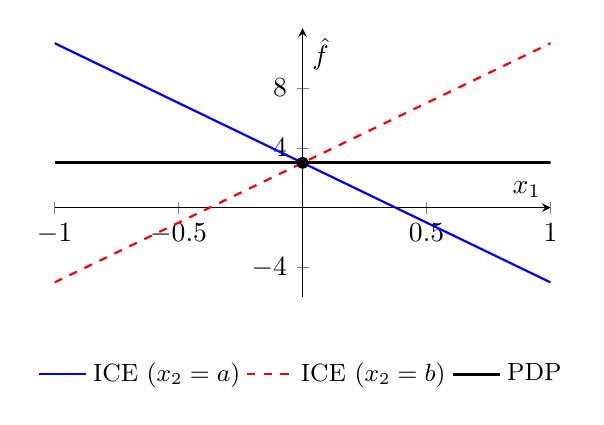
\begin{tikzpicture}
      \begin{axis}[
        width=0.65\textwidth,
        height=5.0cm,
        xmin=-1, xmax=1,
        ymin=-6, ymax=12,
        axis lines=middle,
        xlabel={$x_1$}, ylabel={$\hat f$},
        xtick={-1,-0.5,0,0.5,1},
        ytick={-8,-4,0,4,8},
        samples=101,
        domain=-1:1,
        legend style={draw=none,at={(0.5,-0.2)},anchor=north,legend columns=3,font=\small}
      ]
        \addplot[blue, thick] {-8*x + 3}; \addlegendentry{ICE ($x_2=a$)}
        \addplot[red, thick, dashed] {8*x + 3}; \addlegendentry{ICE ($x_2=b$)}
        \addplot[black, very thick] {3}; \addlegendentry{PDP}
        \addplot[only marks, mark=*, mark size=2pt] coordinates {(0,3)};
      \end{axis}
    \end{tikzpicture}
  \end{figure}

  \item \textbf{Real-world PDP (Bike sharing).} Example (temperature):
  \begin{itemize}
    \item \emph{Rising region:} Rentals grow as temperature moves from cold toward mild (comfort increases).
    \item \emph{Plateau:} Beyond a threshold, additional warmth adds little (diminishing returns).
    \item \emph{Possible masked interactions:} Season (winter suppresses mid temps), hour (commute spikes), humidity (hot+humid lowers comfort).
    \item \emph{Sparse extremes / uncertainty:} Very high temperatures occur rarely (few or no observations near the right edge, visible by x tick spacing / absence of data markers). PDP values there rely on extrapolation from little data, so the far-right tail is less reliable.
  \end{itemize}

  \item \textbf{Correlated features (unrealistic PDP points).}
  \begin{enumerate}
    \item If $x_1$ and $x_3$ are strongly correlated, replacing $x_1$ with grid values while keeping $x_3$ fixed produces \emph{out-of-support} pairs (rare or impossible combinations); e.g. very high temperatures in January.
    \item Unrealistic observations caused by correlated features can make a PDP misleading, since the model's predictions for those impossible feature combinations do not reflect its true behavior on real data.
  \item Mitigations (two concise): (i) Conditional PDP: average predictions using samples drawn from the conditional distribution $p(x_1\mid x_3)$ so only realistic pairs contribute. (ii) ALE: see details below.
  \end{enumerate}

  \item \textbf{ALE vs PDP.} ALE avoids evaluating the model on unrealistic combinations of correlated features by computing local effects only within regions of the data where observations actually exist, thus respecting the joint feature distribution.
\end{enumerate}

\fi


\end{document}
